% Options for packages loaded elsewhere
% Options for packages loaded elsewhere
\PassOptionsToPackage{unicode}{hyperref}
\PassOptionsToPackage{hyphens}{url}
\PassOptionsToPackage{dvipsnames,svgnames,x11names}{xcolor}
%
\documentclass[
  letterpaper,
  DIV=11,
  numbers=noendperiod]{scrartcl}
\usepackage{xcolor}
\usepackage{amsmath,amssymb}
\setcounter{secnumdepth}{-\maxdimen} % remove section numbering
\usepackage{iftex}
\ifPDFTeX
  \usepackage[T1]{fontenc}
  \usepackage[utf8]{inputenc}
  \usepackage{textcomp} % provide euro and other symbols
\else % if luatex or xetex
  \usepackage{unicode-math} % this also loads fontspec
  \defaultfontfeatures{Scale=MatchLowercase}
  \defaultfontfeatures[\rmfamily]{Ligatures=TeX,Scale=1}
\fi
\usepackage{lmodern}
\ifPDFTeX\else
  % xetex/luatex font selection
\fi
% Use upquote if available, for straight quotes in verbatim environments
\IfFileExists{upquote.sty}{\usepackage{upquote}}{}
\IfFileExists{microtype.sty}{% use microtype if available
  \usepackage[]{microtype}
  \UseMicrotypeSet[protrusion]{basicmath} % disable protrusion for tt fonts
}{}
\makeatletter
\@ifundefined{KOMAClassName}{% if non-KOMA class
  \IfFileExists{parskip.sty}{%
    \usepackage{parskip}
  }{% else
    \setlength{\parindent}{0pt}
    \setlength{\parskip}{6pt plus 2pt minus 1pt}}
}{% if KOMA class
  \KOMAoptions{parskip=half}}
\makeatother
% Make \paragraph and \subparagraph free-standing
\makeatletter
\ifx\paragraph\undefined\else
  \let\oldparagraph\paragraph
  \renewcommand{\paragraph}{
    \@ifstar
      \xxxParagraphStar
      \xxxParagraphNoStar
  }
  \newcommand{\xxxParagraphStar}[1]{\oldparagraph*{#1}\mbox{}}
  \newcommand{\xxxParagraphNoStar}[1]{\oldparagraph{#1}\mbox{}}
\fi
\ifx\subparagraph\undefined\else
  \let\oldsubparagraph\subparagraph
  \renewcommand{\subparagraph}{
    \@ifstar
      \xxxSubParagraphStar
      \xxxSubParagraphNoStar
  }
  \newcommand{\xxxSubParagraphStar}[1]{\oldsubparagraph*{#1}\mbox{}}
  \newcommand{\xxxSubParagraphNoStar}[1]{\oldsubparagraph{#1}\mbox{}}
\fi
\makeatother


\usepackage{longtable,booktabs,array}
\newcounter{none} % for unnumbered tables
\usepackage{calc} % for calculating minipage widths
% Correct order of tables after \paragraph or \subparagraph
\usepackage{etoolbox}
\makeatletter
\patchcmd\longtable{\par}{\if@noskipsec\mbox{}\fi\par}{}{}
\makeatother
% Allow footnotes in longtable head/foot
\IfFileExists{footnotehyper.sty}{\usepackage{footnotehyper}}{\usepackage{footnote}}
\makesavenoteenv{longtable}
\usepackage{graphicx}
\makeatletter
\newsavebox\pandoc@box
\newcommand*\pandocbounded[1]{% scales image to fit in text height/width
  \sbox\pandoc@box{#1}%
  \Gscale@div\@tempa{\textheight}{\dimexpr\ht\pandoc@box+\dp\pandoc@box\relax}%
  \Gscale@div\@tempb{\linewidth}{\wd\pandoc@box}%
  \ifdim\@tempb\p@<\@tempa\p@\let\@tempa\@tempb\fi% select the smaller of both
  \ifdim\@tempa\p@<\p@\scalebox{\@tempa}{\usebox\pandoc@box}%
  \else\usebox{\pandoc@box}%
  \fi%
}
% Set default figure placement to htbp
\def\fps@figure{htbp}
\makeatother





\setlength{\emergencystretch}{3em} % prevent overfull lines

\providecommand{\tightlist}{%
  \setlength{\itemsep}{0pt}\setlength{\parskip}{0pt}}



 


\KOMAoption{captions}{tableheading}
\usepackage{tabularx}
\usepackage{float}
\makeatletter
\@ifpackageloaded{caption}{}{\usepackage{caption}}
\AtBeginDocument{%
\ifdefined\contentsname
  \renewcommand*\contentsname{Table of contents}
\else
  \newcommand\contentsname{Table of contents}
\fi
\ifdefined\listfigurename
  \renewcommand*\listfigurename{List of Figures}
\else
  \newcommand\listfigurename{List of Figures}
\fi
\ifdefined\listtablename
  \renewcommand*\listtablename{List of Tables}
\else
  \newcommand\listtablename{List of Tables}
\fi
\ifdefined\figurename
  \renewcommand*\figurename{Figure}
\else
  \newcommand\figurename{Figure}
\fi
\ifdefined\tablename
  \renewcommand*\tablename{Table}
\else
  \newcommand\tablename{Table}
\fi
}
\@ifpackageloaded{float}{}{\usepackage{float}}
\floatstyle{ruled}
\@ifundefined{c@chapter}{\newfloat{codelisting}{h}{lop}}{\newfloat{codelisting}{h}{lop}[chapter]}
\floatname{codelisting}{Listing}
\newcommand*\listoflistings{\listof{codelisting}{List of Listings}}
\makeatother
\makeatletter
\makeatother
\makeatletter
\@ifpackageloaded{caption}{}{\usepackage{caption}}
\@ifpackageloaded{subcaption}{}{\usepackage{subcaption}}
\makeatother
\usepackage{bookmark}
\IfFileExists{xurl.sty}{\usepackage{xurl}}{} % add URL line breaks if available
\urlstyle{same}
\hypersetup{
  pdftitle={Report of Sri Lanka Dengue Dashboard},
  pdfauthor={Y.M. Amali P. Rajapaksha},
  colorlinks=true,
  linkcolor={blue},
  filecolor={Maroon},
  citecolor={Blue},
  urlcolor={Blue},
  pdfcreator={LaTeX via pandoc}}


\title{Report of Sri Lanka Dengue Dashboard}
\author{Y.M. Amali P. Rajapaksha}
\date{2026-07-08}
\begin{document}
\maketitle


This dashboard provides an interactive overview of the dengue situation
in Sri Lanka using the latest available surveillance data. Built with R
using the Quarto Dashboard framework, it presents recent dengue trends,
district-level analyses, historical patterns, comparisons with the
global dengue situation, and explores the relationship between dengue
transmission and key climate variables. The dashboard offers valuable
insights for monitoring, understanding, and supporting evidence-based
decision-making on dengue dynamics in Sri Lanka.

\subsection{Dashboard Link}\label{dashboard-link}

\url{https://amalirajapaksha.github.io/denguedashboard_SriLanka/}

\subsection{Created By}\label{created-by}

Name : Y.M.A.P. Rajapaksha

Index No : AS2022642

\subsection{Data}\label{data}

\begin{itemize}
\item
  All local data up to December 2025 used in this dashboard are obtained
  from the weekly epidemiological reports published by the Epidemiology
  Unit, Ministry of Health, Sri Lanka, through the
  \texttt{denguedatahub} R package, available at
  https://github.com/thiyangt/denguedatahub.
\item
  Data for 2026 are obtained from the weekly epidemiological reports
  published by the Epidemiology Unit, Ministry of Health, Sri Lanka, and
  the Weekly Dengue Updates published by the National Dengue Control
  Unit, Ministry of Health, Sri Lanka. These data are extracted through
  web scraping using the \texttt{convert\_slwer\_to\_tidy()} function
  available in the \texttt{denguedatahub} package. The processed
  datasets are available in
  \texttt{data/sri\_lanka\_weekly\_dengue\_cases\_2026.csv} and
  \texttt{data/last\_week\_comparisson.xlsx}.
\item
  The global data used in this dashboard are obtained from the World
  Health Organization's
  \href{https://worldhealthorg.shinyapps.io/dengue_global/}{Global
  Dengue Surveillance Dashboard}. The corresponding dataset is available
  in \texttt{data/dengue-global-data.xlsx}.
\item
  The climate data used in this study were downloaded from the
  \href{https://power.larc.nasa.gov/data-access-viewer/}{NASA POWER Data
  Access Viewer}, provided by the National Aeronautics and Space
  Administration (NASA). The processed weekly climate dataset is
  available in \texttt{data/weekly\_climate.csv}.
\item
  All raw data files are available in the \texttt{raw-data} directory.
\item
  All R scripts used for data preprocessing are available in the
  \texttt{pre\_processing} directory.
\end{itemize}

\subsection{Methodology}\label{methodology}

Here, several visualization techniques have been used for different
purposes. To explore new visualization techniques that can be applied
for disease surveillance and epidemiological analysis, the
\href{https://thiyangt.github.io/coviddashboard/}{Sri Lanka COVID-19
Dashboard} (Talagala \& De Alwis, 2021) was referred to. To get an
overall idea of the methodologies, see Table 1.

\begin{table}[H]
\centering
\caption{Summary of methodologies used in the dashboard}
\begin{tabularx}{\textwidth}{|X|p{4cm}|}
\hline
\textbf{Information Presented} & \textbf{Visualization Technique(s)} \\
\hline
Key Information about the Present Dengue Situation in Sri Lanka & KPIs \\
\hline
Distribution of Total Dengue Cases in Sri Lanka in 2026 & Choropleth Map \\
\hline
Cumulative Dengue Deaths in Sri Lanka in 2026 & Choropleth Map \\
\hline
Anomalous Dengue Behaviour in the Current Period Compared with the Previous Two Years in Sri Lanka & Time Series Plot \\
\hline
Last Week's Dengue Situation Analysis & Choropleth Maps \\
\hline
District-wise Weekly Dengue Case Analysis Over Time until 2025 & Faceted and Individual Time Series Plots, Faceted and Individual Seasonal Plots \\
\hline
Distribution of Dengue Patients by District and Year until 2025 & Tree map, Faceted Choropleth Map, Heatmap \\
\hline
Relationship Between Climatic Variables and Dengue Cases & Multi-panel Time Series Plot, Scatterplots \\
\hline
Global Distribution of Dengue Patients/Cases in 2025 & Choropleth Map \\
\hline
Sri Lanka Compared with the Top 10 Dengue-Affected Countries Worldwide and Other South-East Asian countries in 2025 & Stacked Bar Chart \\
\hline
\end{tabularx}
\end{table}

One of the additional analyses included in this dashboard is the
climate-dengue relationship analysis. In addition to time series plots
(Figure 6.a) and scatter plots (Figure 6.b) of climatic variables
vs.~dengue cases, I explored the potential lag effect using two-week and
four-week lag scatter plots (Figure 6.c , Figure 6.d). Dengue
transmission does not respond immediately to climatic changes such as
rainfall and humidity. Instead, favourable climatic conditions may
enhance mosquito breeding and contribute to increased dengue cases after
a certain time lag. Based on this idea, I explored the lag relationship
between climatic factors and dengue cases. Furthermore, to obtain a
comprehensive understanding of the relationship between climatic
variables and dengue cases, the Detrended Cross-Correlation Coefficient
(\(\rho_{DCCA}\)) was calculated across different time scales (Figueredo
et al., 2023). This method is used to study the relationship between
multiple time series that change over time, even when the data are not
stationary (Zebende et al., 2018). The calculated \(\rho_{DCCA}\) values
were plotted over different time scales to investigate how climatic
variables influence dengue occurrence across short, medium and long-term
periods.

In this dashboard, several colour palettes were used ensuring that the
visualizations are colour-blind friendly. These include the Viridis
palette from the viridis package (Garnier et al., 2024), the Paired
palette from the ColorBrewer collection (Brewer, 2003), and the Magma
palette from the Viridis colour map family (van der Walt \& Smith,
2015). In addition, some colour themes were manually defined according
to the context of the visualizations.

In this dashboard, multiple visualization techniques have sometimes been
used for the same data. Although the data are the same, each
visualization provides different insights that can be directly obtained
from the data. Therefore, using multiple plots for the same data helps
explore different aspects of the actual situation more comprehensively.

\subsection{Results}\label{results}

\begin{figure}[H]

\centering{

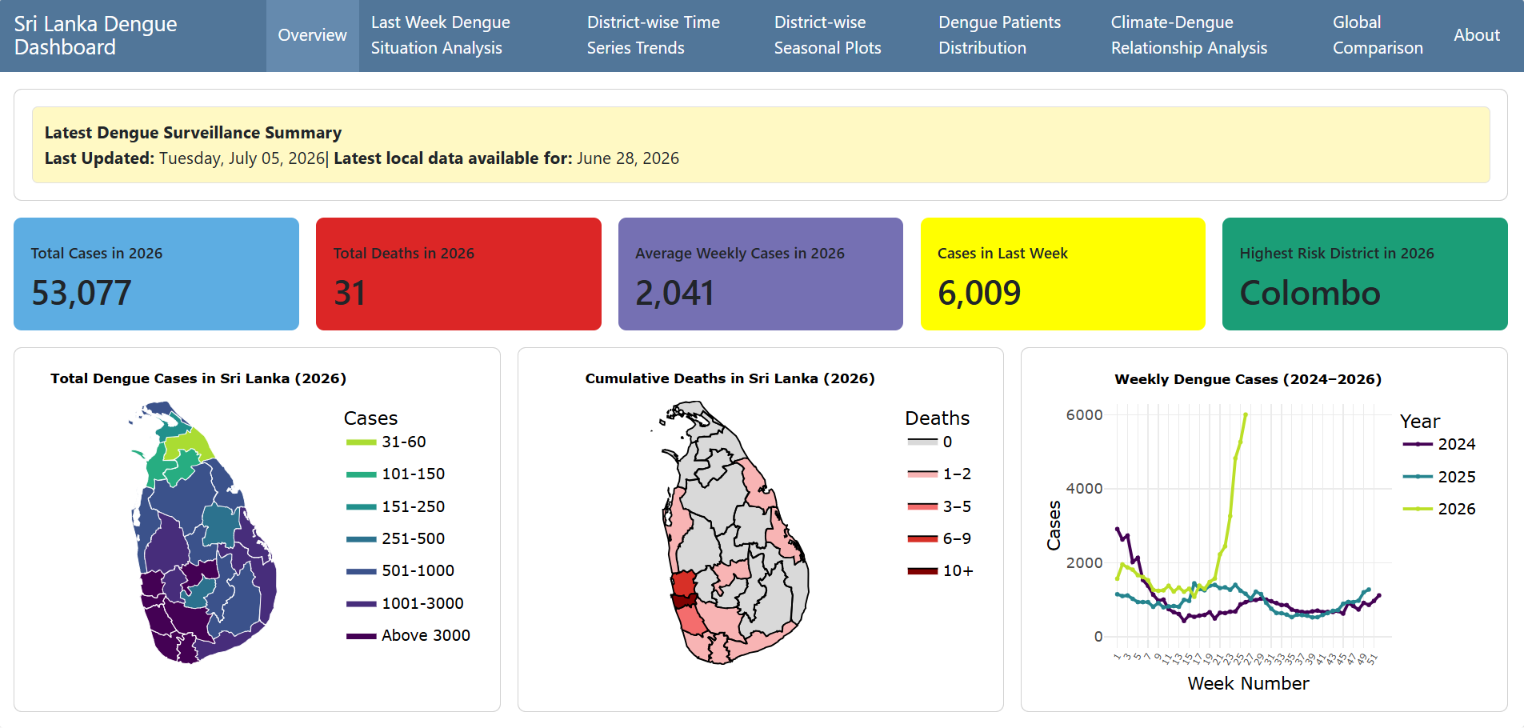
\includegraphics[width=5.08in,height=\textheight,keepaspectratio]{images/tab1.png}

}

\caption{\label{fig-tab1}Screenshot of Tab 1 (Overview)}

\end{figure}%

The dashboard is organized into 8 navigation tabs, including Overview,
Last Week Dengue Situation Analysis, District-wise Time Series Trends,
District-wise Seasonal Plots, Dengue Patients Distribution,
Climate-Dengue Relationship Analysis, Global Comparison, and About. Each
tab contains interactive visualizations and analytical outputs. Table 2
provides a description of each tab and summarizes its key content.

\begin{table}[H]
\centering
\caption{Description of Dashboard Tabs}
\begin{tabularx}{\textwidth}{|p{2cm}|X|}
\hline
\textbf{Tab No.} & \textbf{Description} \\
\hline
Tab 1 & This provides the latest information about the dengue epidemic in Sri Lanka. It gives a brief overview of the current dengue situation in Sri Lanka. \\
\hline
Tab 2 & This compares the dengue situation in the 26th week of this year with the same week of the previous year. This is the latest data we have. \\
\hline
Tab 3 & There are two sub-tabs. The first contains faceted time series plots of weekly dengue cases from 2006 to 2025 for each district separately. The second tab allows users to explore small changes in dengue cases for each district individually using dygraphs. \\
\hline
Tab 4 & There are two sub-tabs. The first contains faceted seasonal plots of weekly dengue cases from 2006 to 2025 for each district separately. The second tab allows users to explore small changes in seasonal patterns for each district individually using Plotly graphs. \\
\hline
Tab 5 & There are three sub-tabs. The first contains a treemap showing the distribution of total dengue patients in 2025. The second and third sub-tabs contain the distribution of dengue patients over the last 20 years by district and year.   \\
\hline
Tab 6 & This section contains five sub-tabs and provides a comprehensive analysis of the relationship between climatic variables and dengue cases. The first four sub-tabs present time series plots and scatter plots to explore temporal patterns and associations between climatic variables and dengue incidence. The fifth sub-tab presents a map displaying the calculated raw DCCA values across different time scales.\\
\hline
Tab 7 & This section has three sub-tabs. The first shows the distribution of dengue patients worldwide in 2025. The second and third sub-tabs compare the dengue situation in Sri Lanka with the global and South-East Asia region levels, respectively. \\
\hline
Tab 8 & This contains detailed information about the dashboard, data sources, references, and other related information. \\
\hline
\end{tabularx}
\end{table}

According to Figure 1, a rapid increase in dengue cases can be observed
in 2026 from around the 21st week compared with 2024 and 2025. Public
sources suggest that this increase may be associated with enhanced Aedes
mosquito breeding due to favourable climatic conditions, post-flood
environmental changes following Cyclone Ditwah, urbanization-related
breeding habitats, and ongoing dengue virus transmission dynamics.

\begin{figure}[H]

\centering{

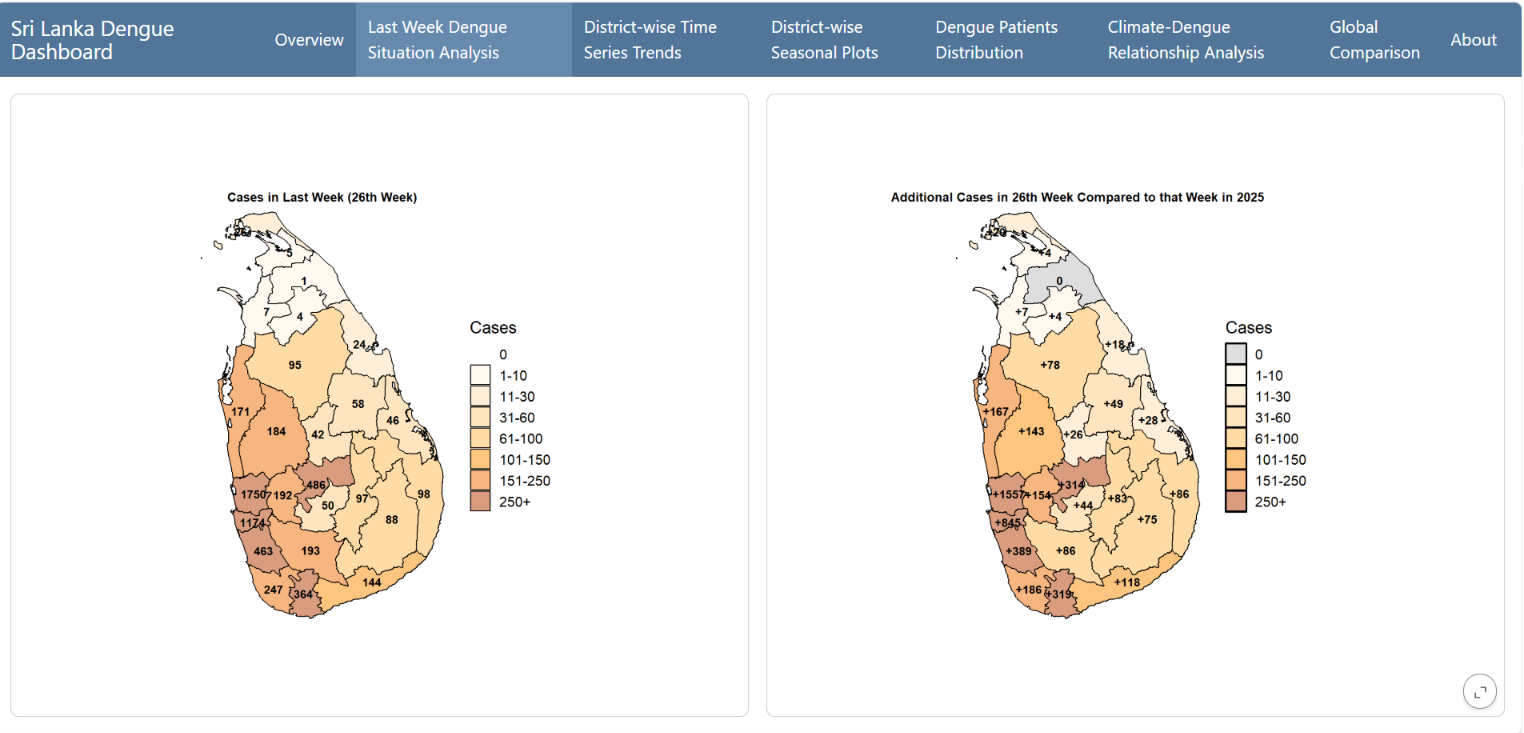
\includegraphics[width=5.08in,height=\textheight,keepaspectratio]{images/tab2.png}

}

\caption{\label{fig-tab2}Screenshot of Tab 2 (Last Week Dengue Situation
Analysis)}

\end{figure}%

Figure 2 also proves the severity of the situation Sri Lanka faces
today. Approximately, the number of cases reported in the 26th week this
year is nearly twice that of the same week last year.

\begin{figure}[H]

\begin{minipage}[t]{0.50\linewidth}

\centering{

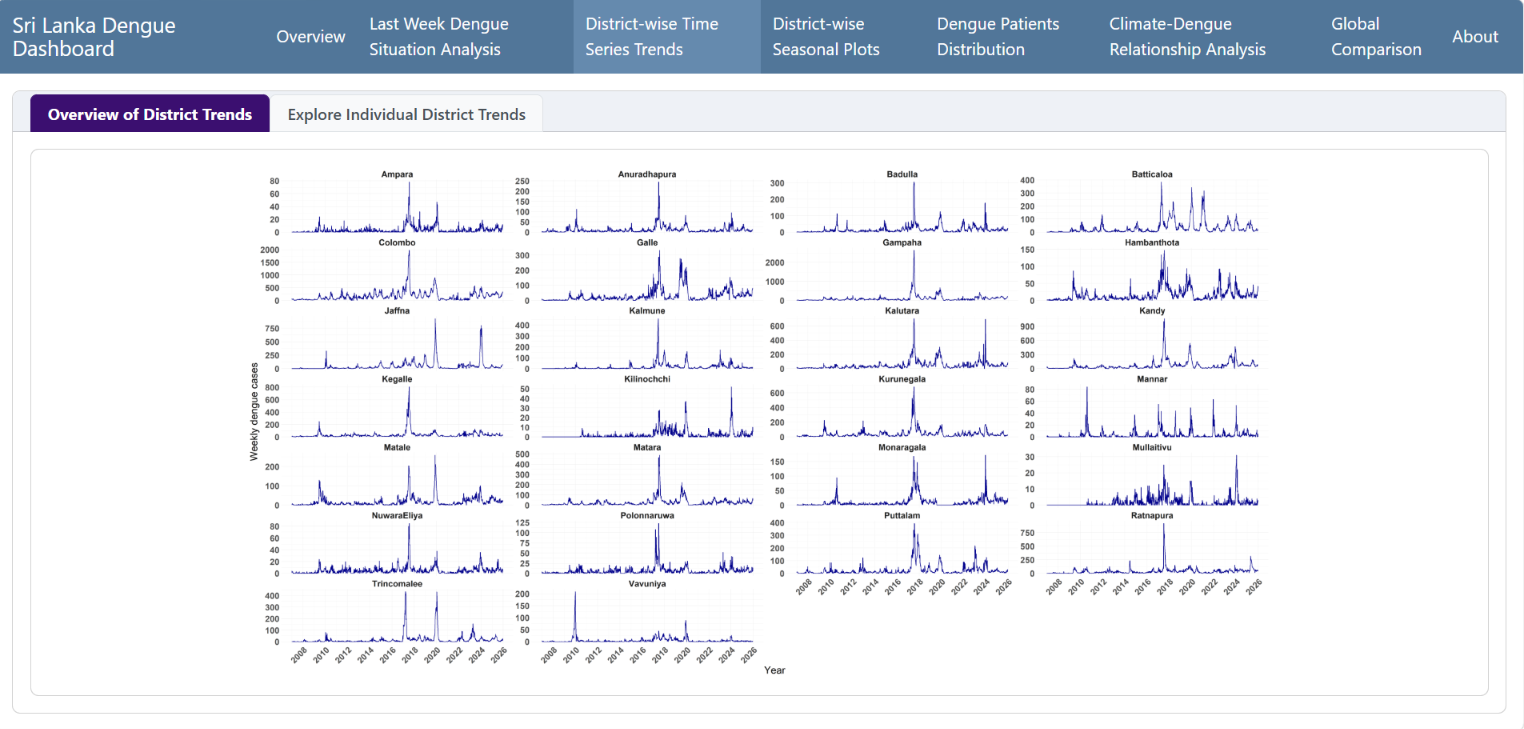
\includegraphics[width=0.98\linewidth,height=\textheight,keepaspectratio]{images/tab3.a.png}

}

\subcaption{\label{fig-tab3-1}}

\end{minipage}%
%
\begin{minipage}[t]{0.50\linewidth}

\centering{

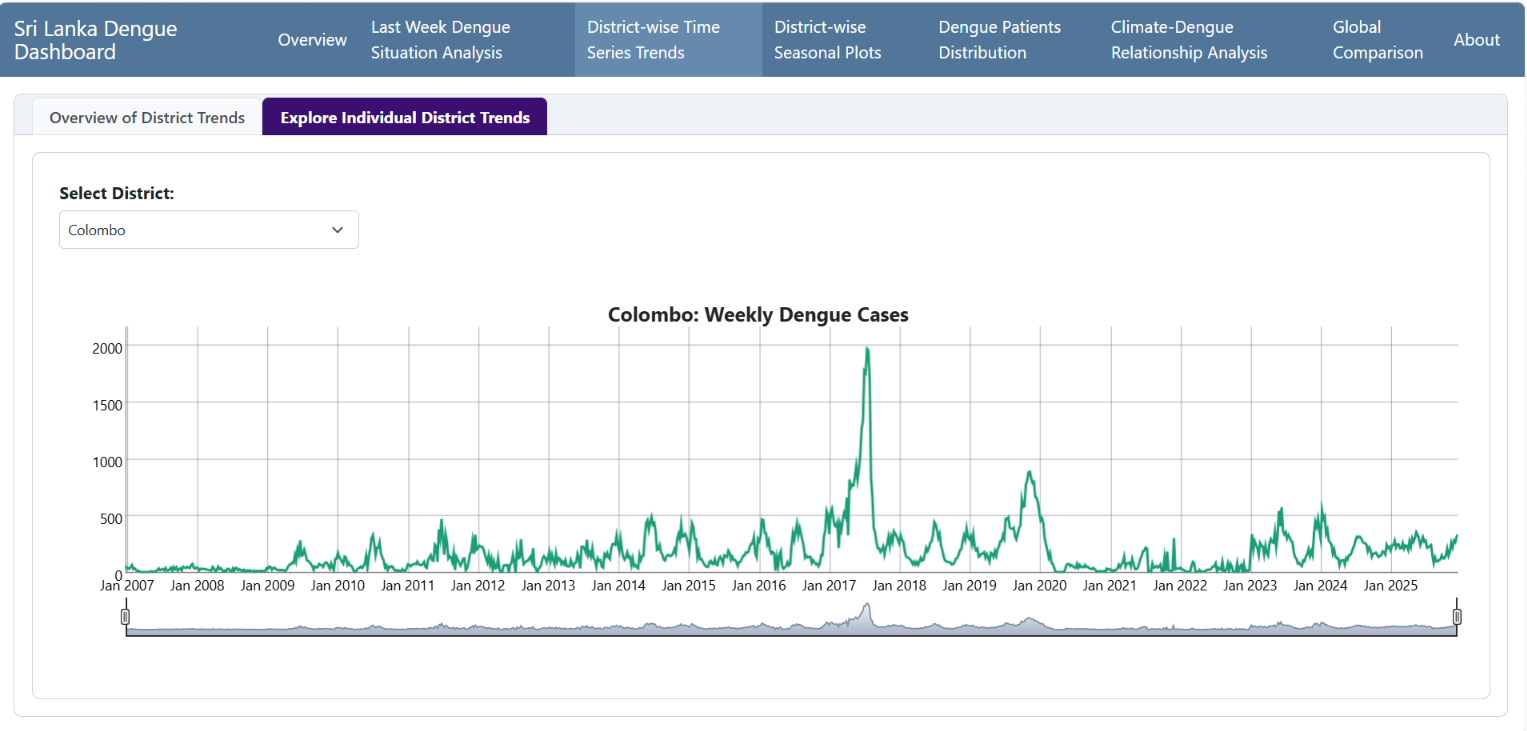
\includegraphics[width=0.98\linewidth,height=\textheight,keepaspectratio]{images/tab3.b.png}

}

\subcaption{\label{fig-tab3-2}}

\end{minipage}%

\caption{\label{fig-tab3}Screenshot of Tab 3 (District-wise Time Series
Trends)}

\end{figure}%

Figure 3.a shows that many districts experienced notable peaks in dengue
cases during 2017, 2019, and 2023. Among these, the 2017 outbreak was
the most severe, with consistently high case counts across nearly all
districts. According to published reports, Sri Lanka recorded its
largest dengue outbreak in 2017, with 186,101 suspected cases and 440
deaths nationwide. Preliminary laboratory investigations identified
Dengue virus serotype 2 (DENV-2) as the predominant circulating strain
associated with this outbreak.

\subsection{Tab 4}\label{tab-4}

\begin{figure}[H]

\begin{minipage}[t]{0.50\linewidth}

\centering{

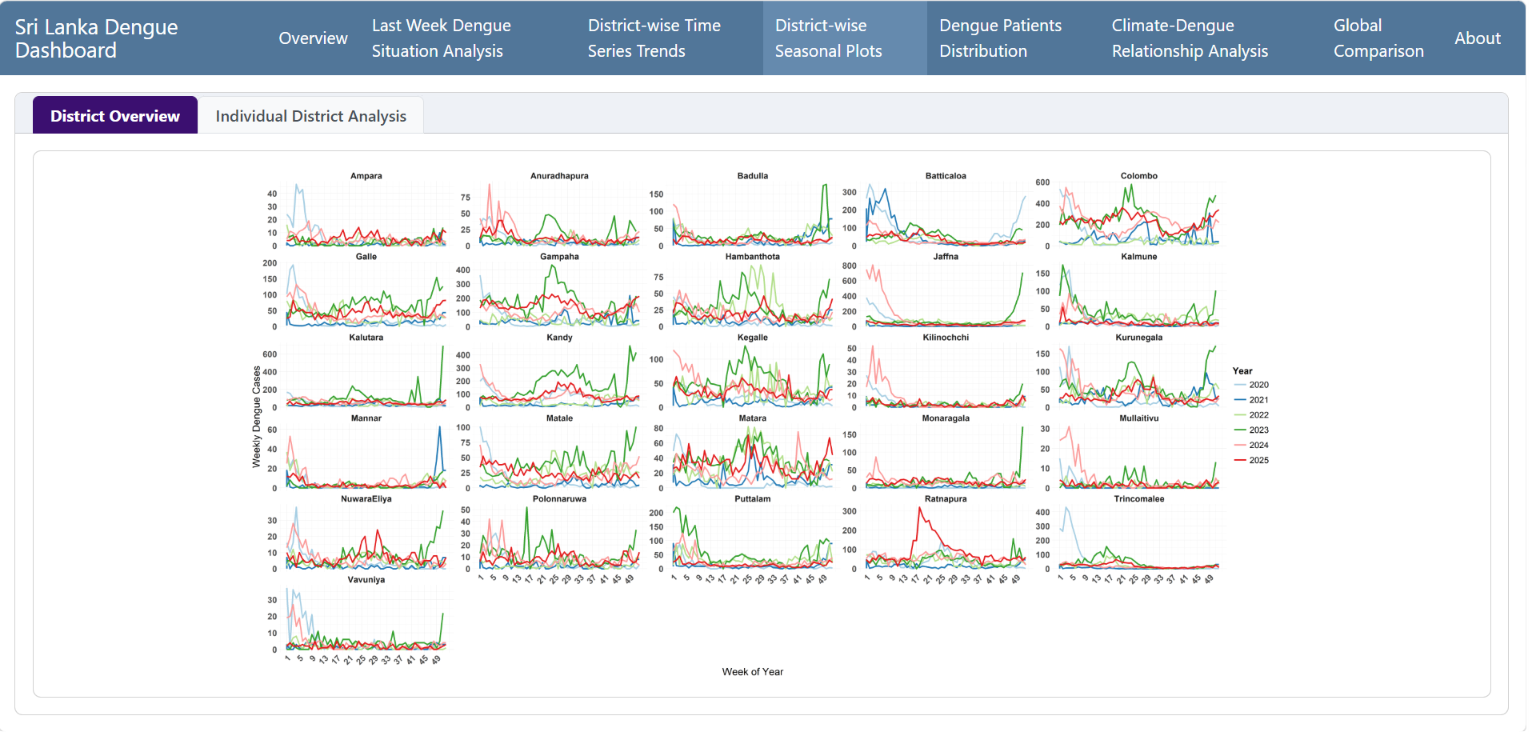
\includegraphics[width=0.98\linewidth,height=\textheight,keepaspectratio]{images/tab4.a.png}

}

\subcaption{\label{fig-tab4-1}}

\end{minipage}%
%
\begin{minipage}[t]{0.50\linewidth}

\centering{

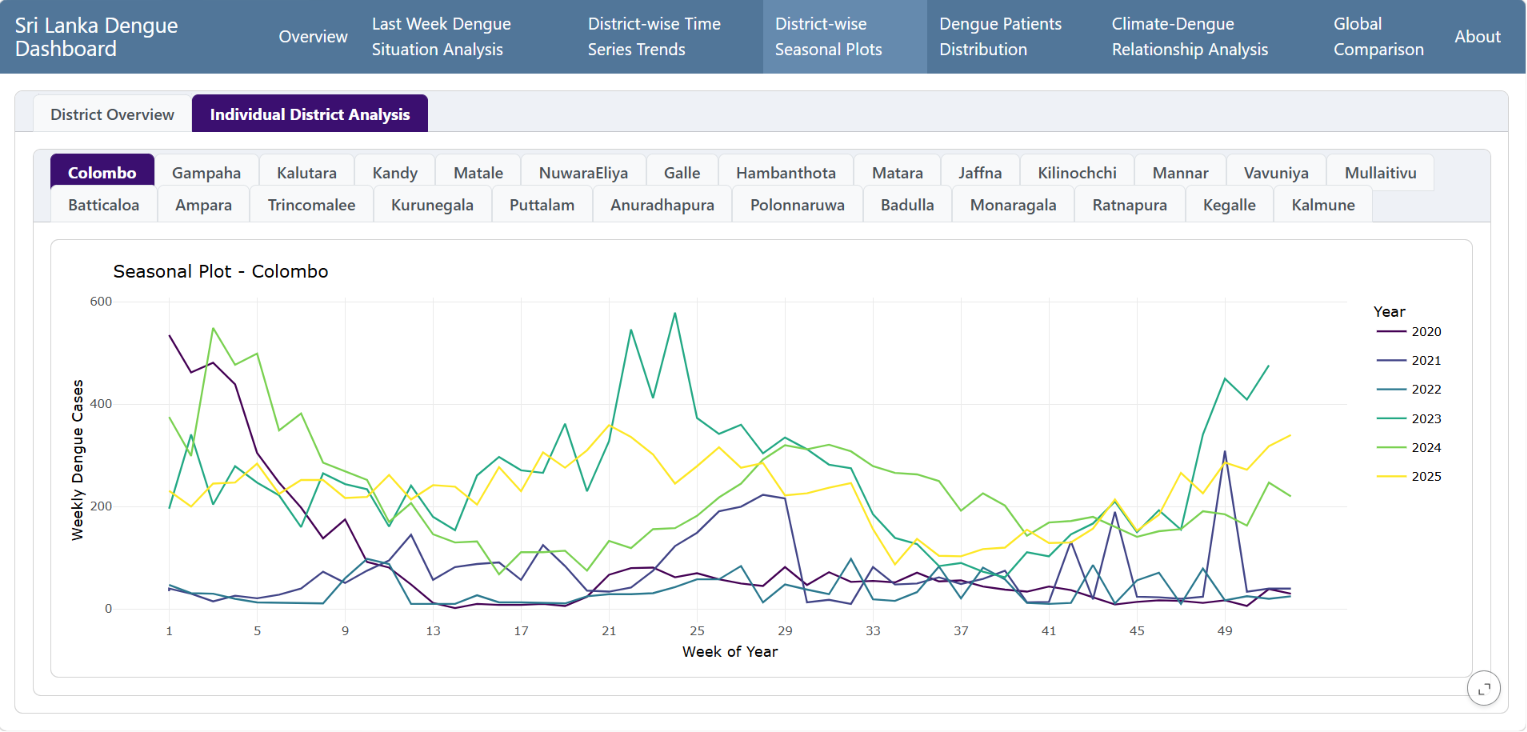
\includegraphics[width=0.98\linewidth,height=\textheight,keepaspectratio]{images/tab4.b.png}

}

\subcaption{\label{fig-tab4-2}}

\end{minipage}%

\caption{\label{fig-tab4}Screenshot of Tab 4 (District-wise Seasonal
Plots)}

\end{figure}%

\subsection{Tab 5}\label{tab-5}

\begin{figure}[H]

\begin{minipage}[t]{0.50\linewidth}

\centering{

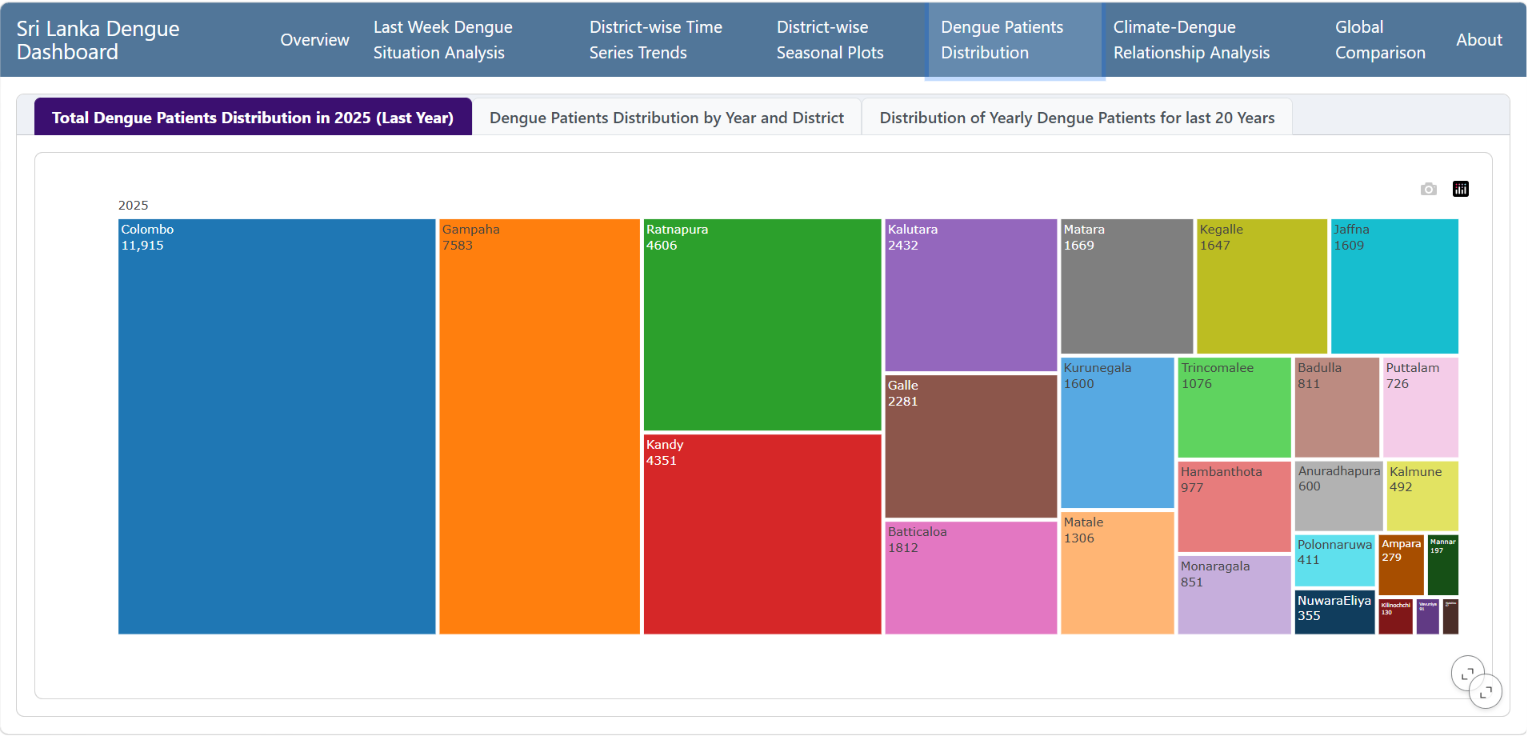
\includegraphics[width=0.98\linewidth,height=\textheight,keepaspectratio]{images/tab5.a.png}

}

\subcaption{\label{fig-tab5-1}}

\end{minipage}%
%
\begin{minipage}[t]{0.50\linewidth}

\centering{

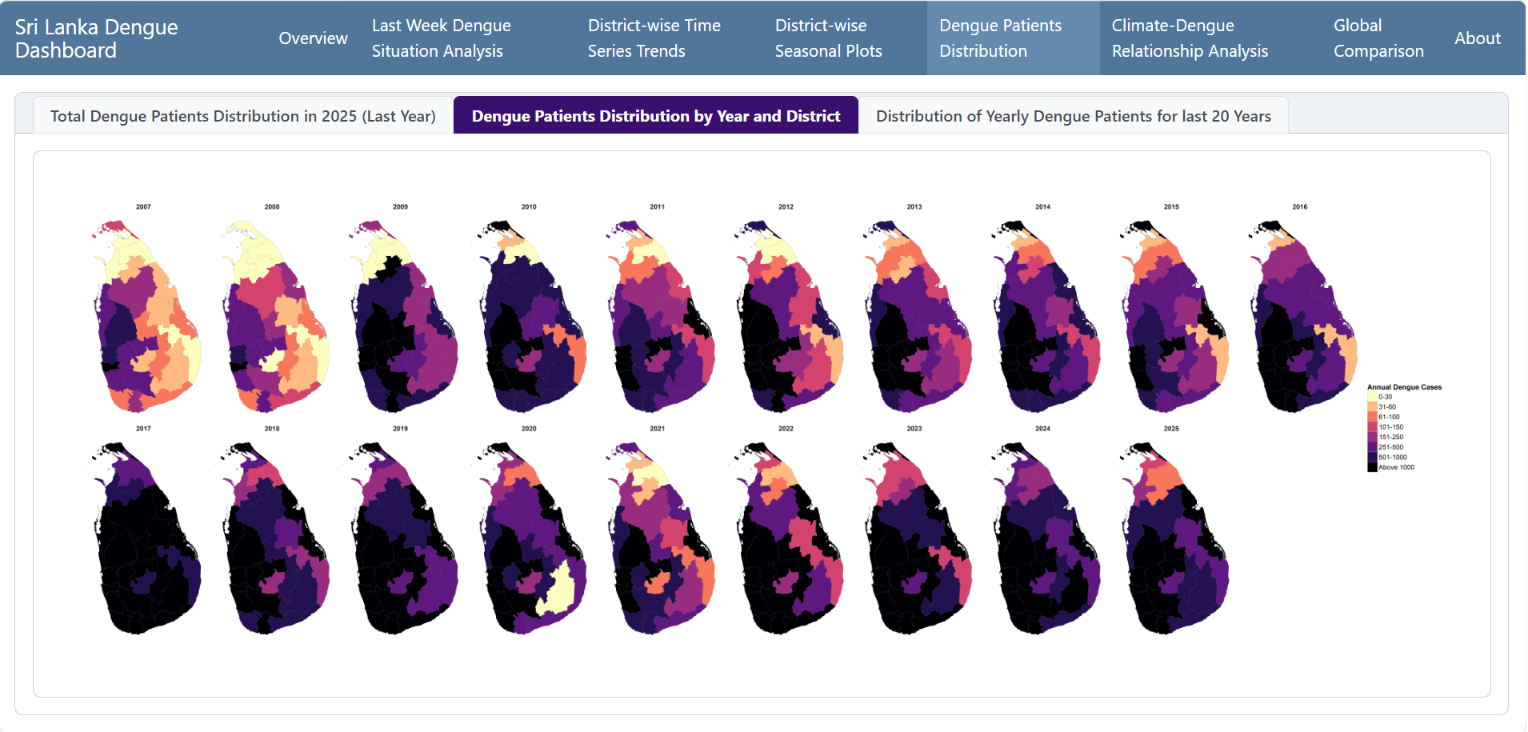
\includegraphics[width=0.98\linewidth,height=\textheight,keepaspectratio]{images/tab5.b.png}

}

\subcaption{\label{fig-tab5-2}}

\end{minipage}%
\newline
\begin{minipage}[t]{0.50\linewidth}

\centering{

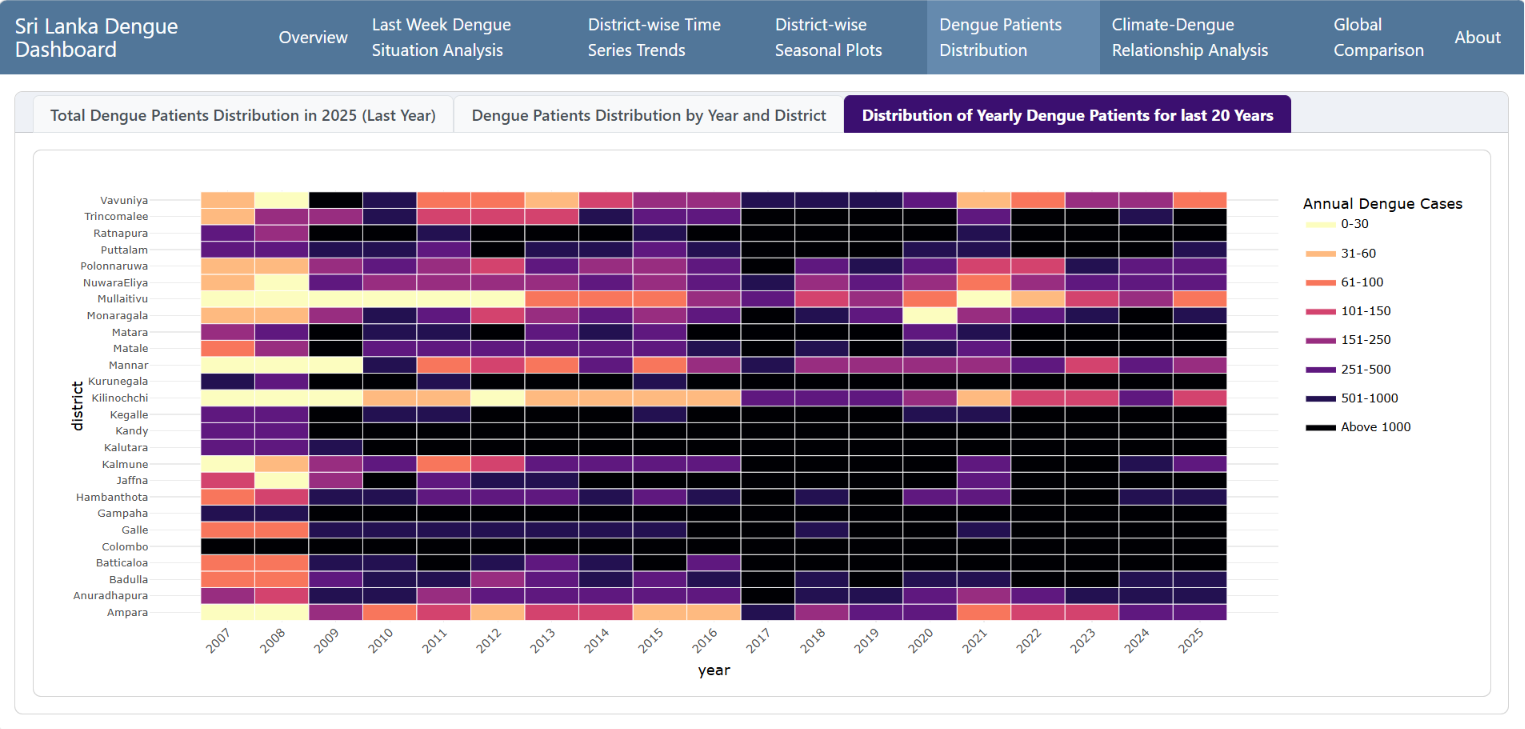
\includegraphics[width=0.98\linewidth,height=\textheight,keepaspectratio]{images/tab5.c.png}

}

\subcaption{\label{fig-tab5-3}}

\end{minipage}%

\caption{\label{fig-tab5}Screenshot of Tab 5 (Dengue Patients
Distribution)}

\end{figure}%

\subsection{Tab 6}\label{tab-6}

\begin{figure}[H]

\begin{minipage}[t]{0.50\linewidth}

\centering{

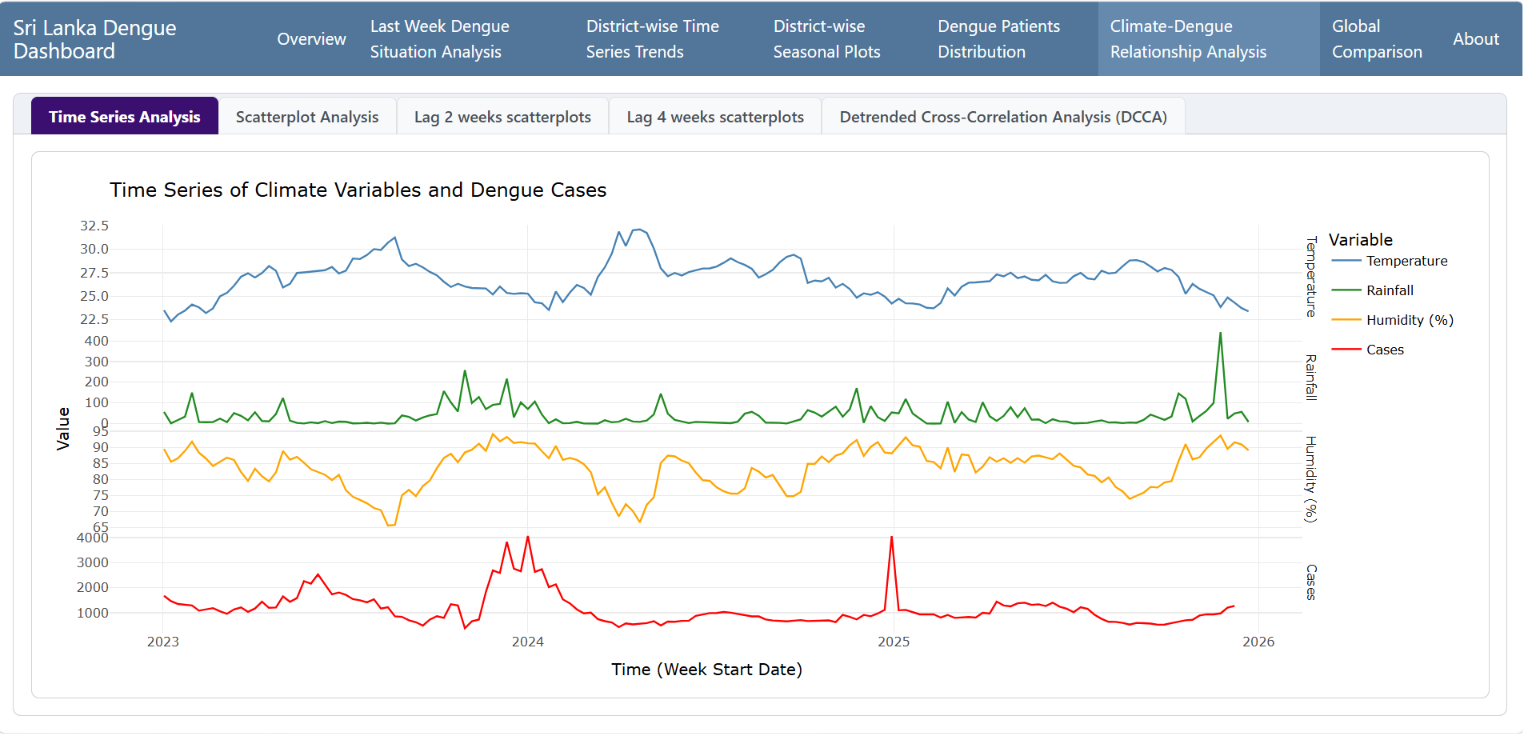
\includegraphics[width=0.98\linewidth,height=\textheight,keepaspectratio]{images/tab6.a.png}

}

\subcaption{\label{fig-tab6-1}}

\end{minipage}%
%
\begin{minipage}[t]{0.50\linewidth}

\centering{

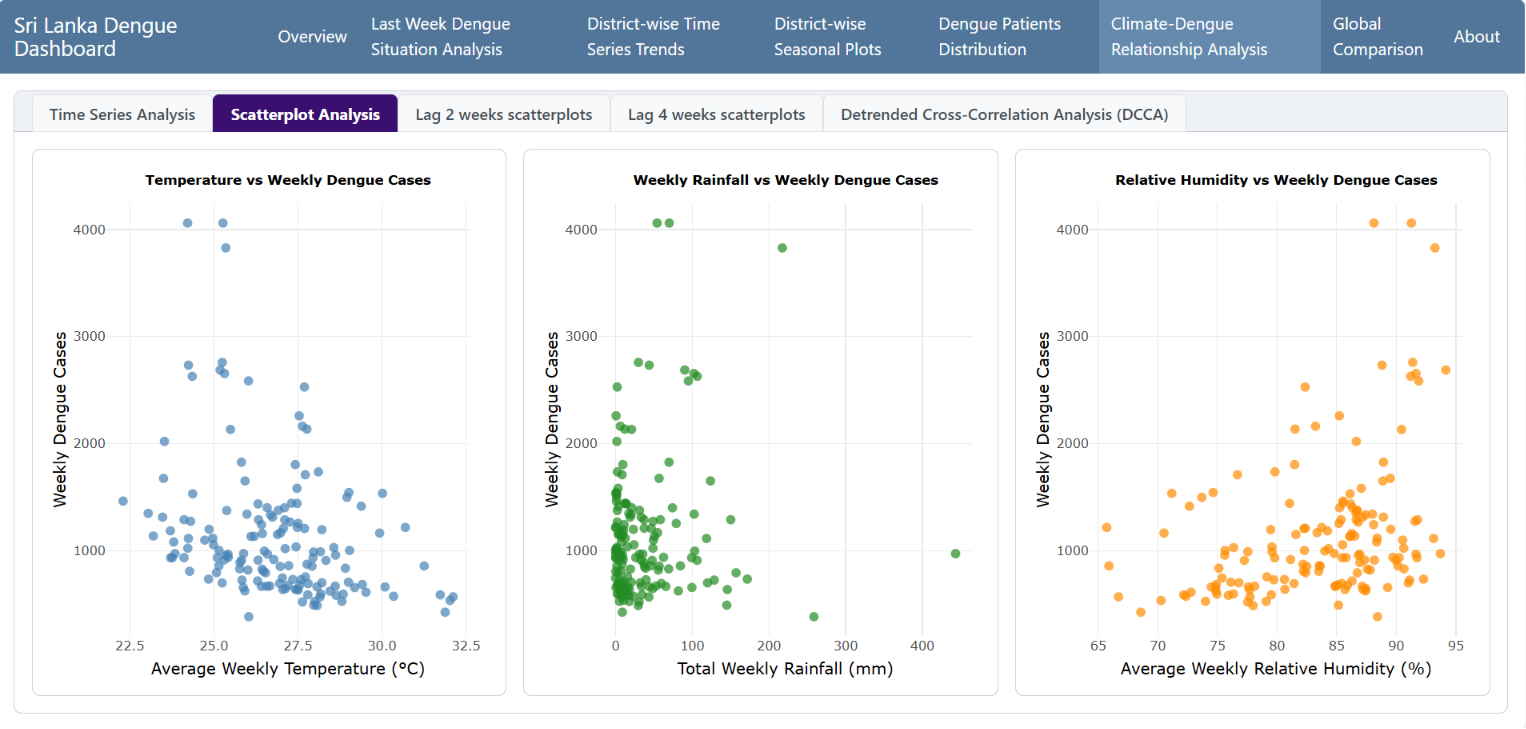
\includegraphics[width=0.98\linewidth,height=\textheight,keepaspectratio]{images/tab6.b.png}

}

\subcaption{\label{fig-tab6-2}}

\end{minipage}%
\newline
\begin{minipage}[t]{0.50\linewidth}

\centering{

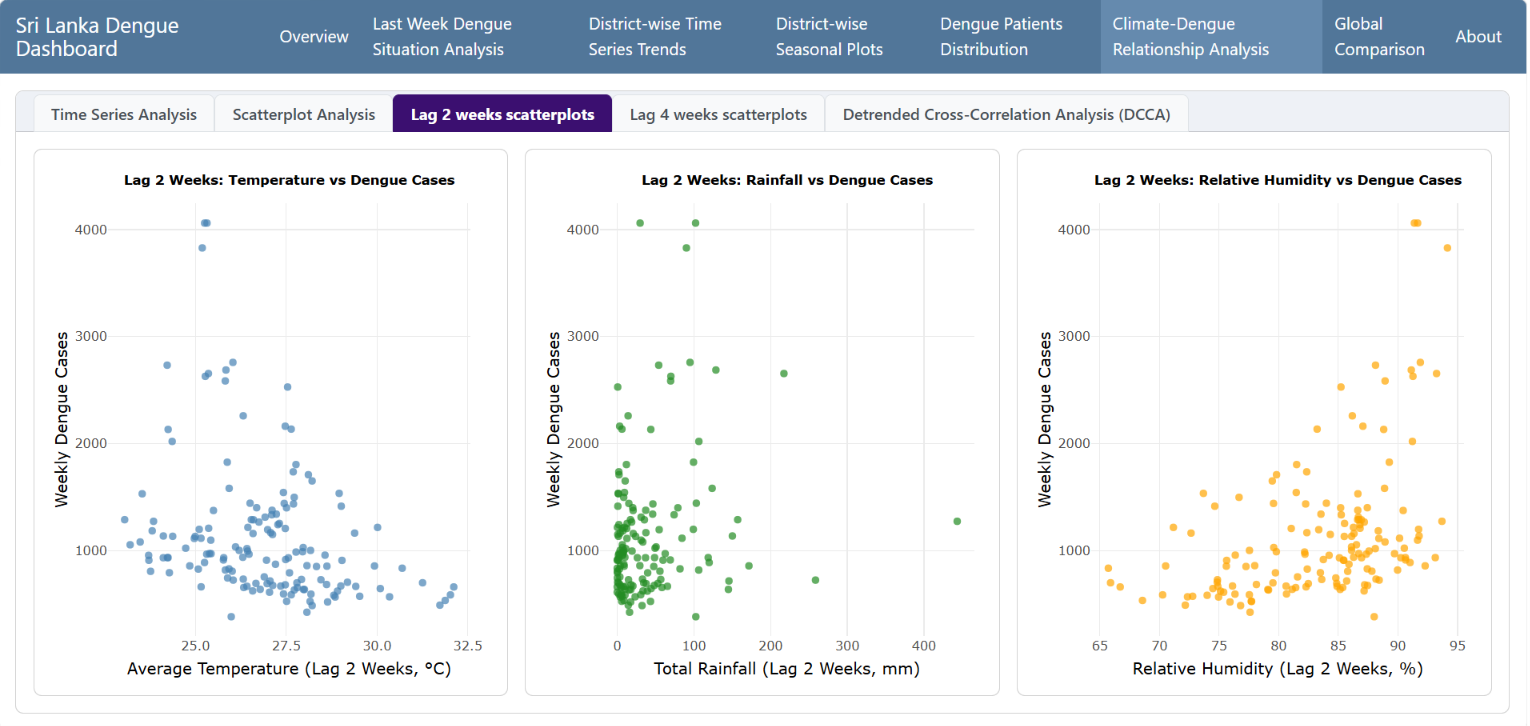
\includegraphics[width=0.98\linewidth,height=\textheight,keepaspectratio]{images/tab6.c.png}

}

\subcaption{\label{fig-tab6-3}}

\end{minipage}%
%
\begin{minipage}[t]{0.50\linewidth}

\centering{

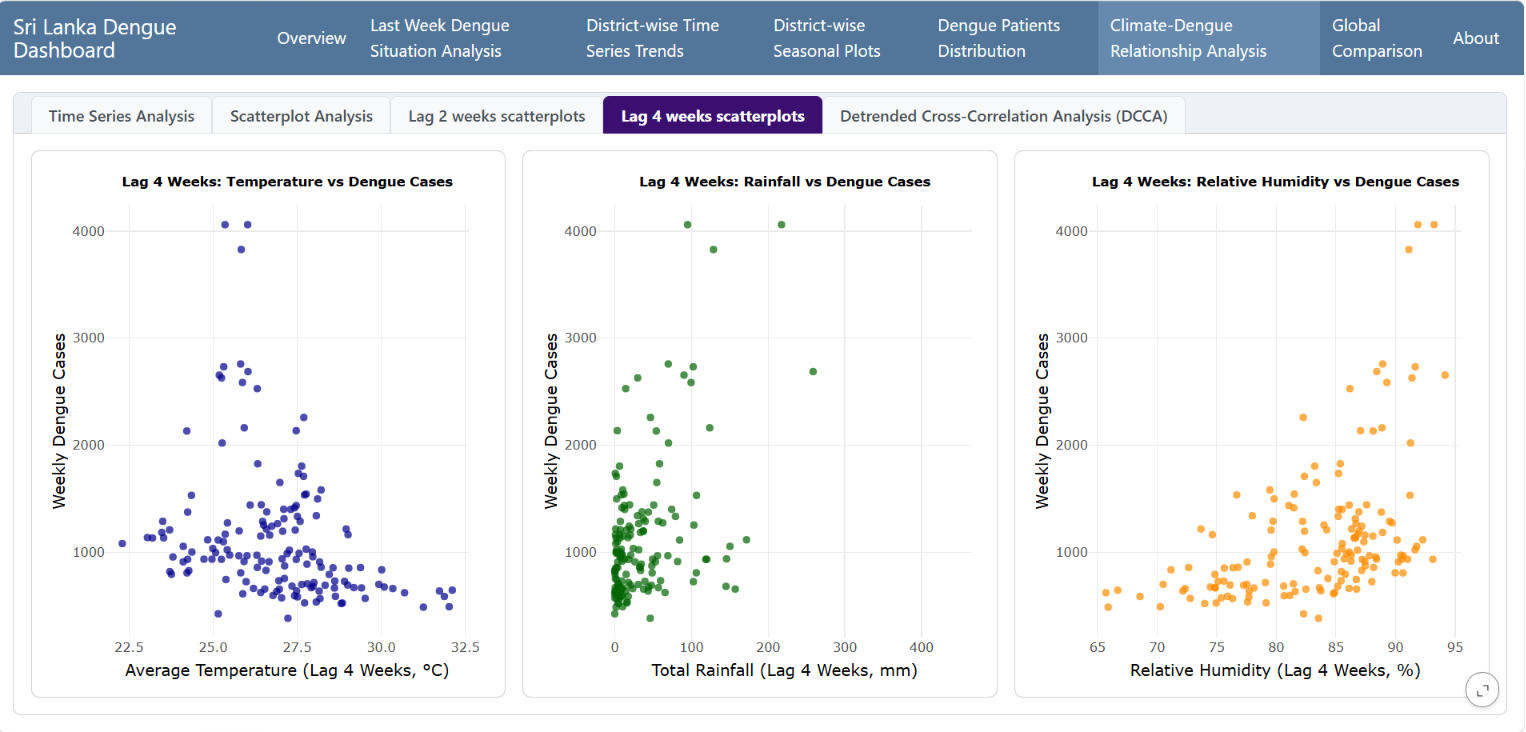
\includegraphics[width=0.98\linewidth,height=\textheight,keepaspectratio]{images/tab6.d.png}

}

\subcaption{\label{fig-tab6-4}}

\end{minipage}%
\newline
\begin{minipage}[t]{0.50\linewidth}

\centering{

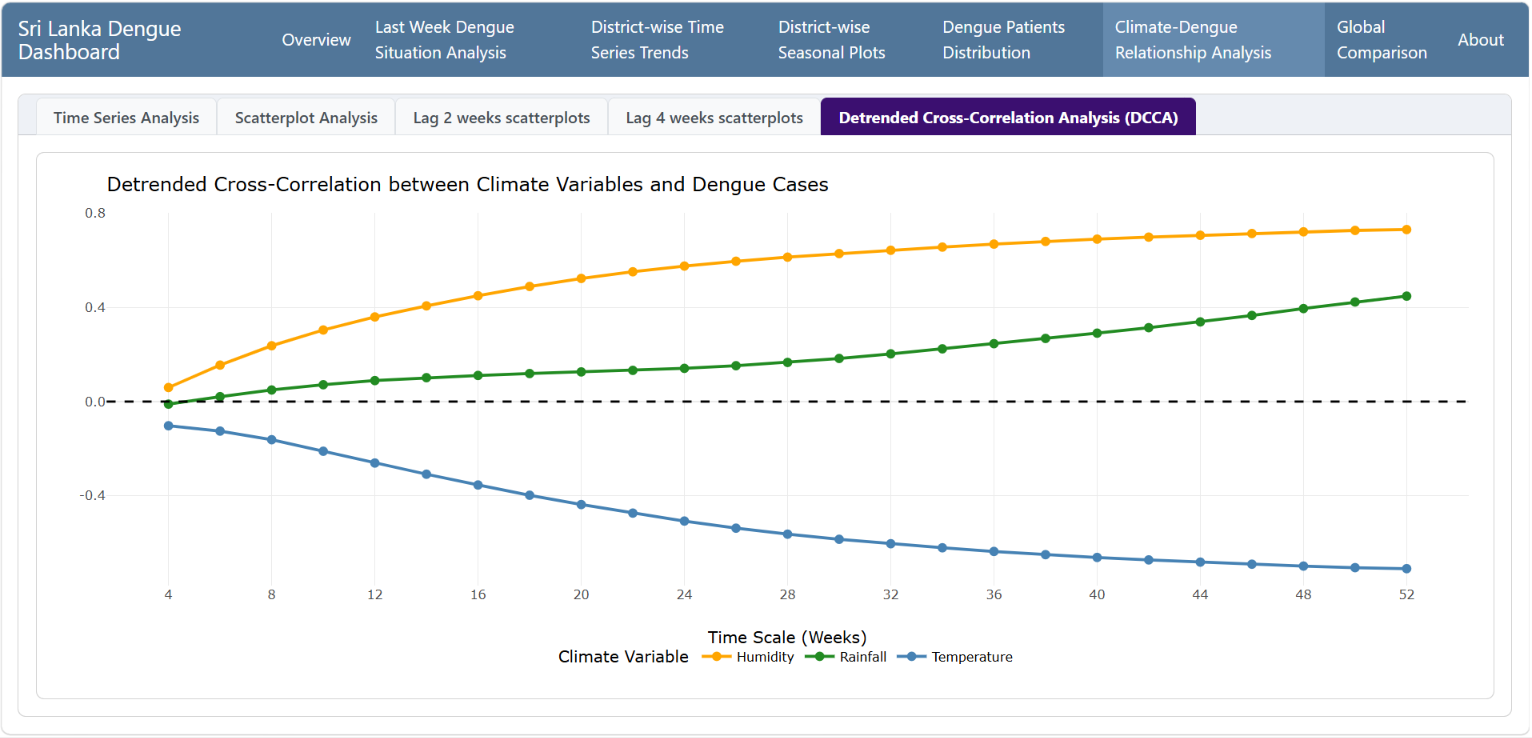
\includegraphics[width=0.98\linewidth,height=\textheight,keepaspectratio]{images/tab6.e.png}

}

\subcaption{\label{fig-tab6-5}}

\end{minipage}%

\caption{\label{fig-tab6}Screenshot of Tab 6 (Climate-Dengue
Relationship Analysis)}

\end{figure}%

\subsection{Tab 7}\label{tab-7}

\begin{figure}[H]

\begin{minipage}[t]{0.50\linewidth}

\centering{

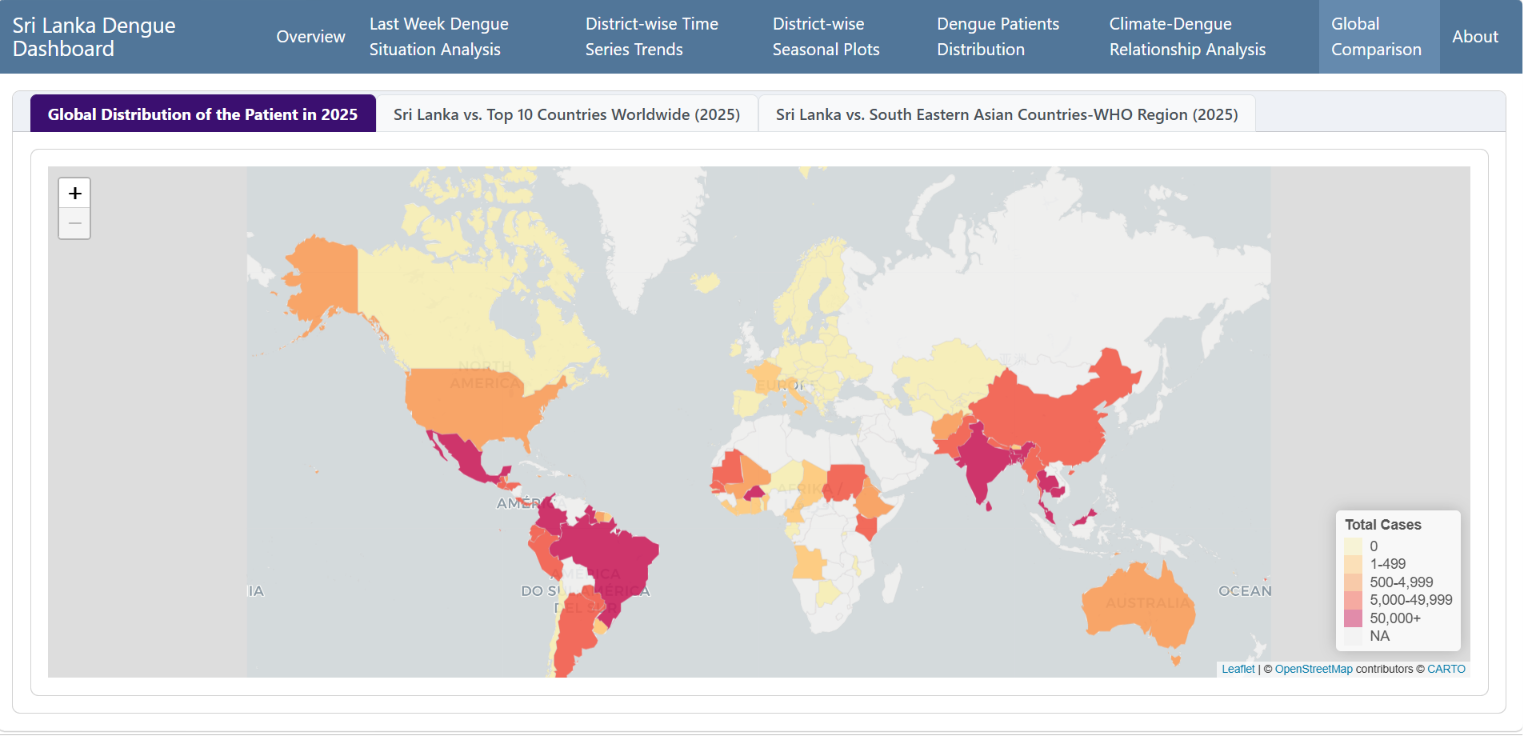
\includegraphics[width=0.98\linewidth,height=\textheight,keepaspectratio]{images/tab7.a.png}

}

\subcaption{\label{fig-tab7-1}}

\end{minipage}%
%
\begin{minipage}[t]{0.50\linewidth}

\centering{

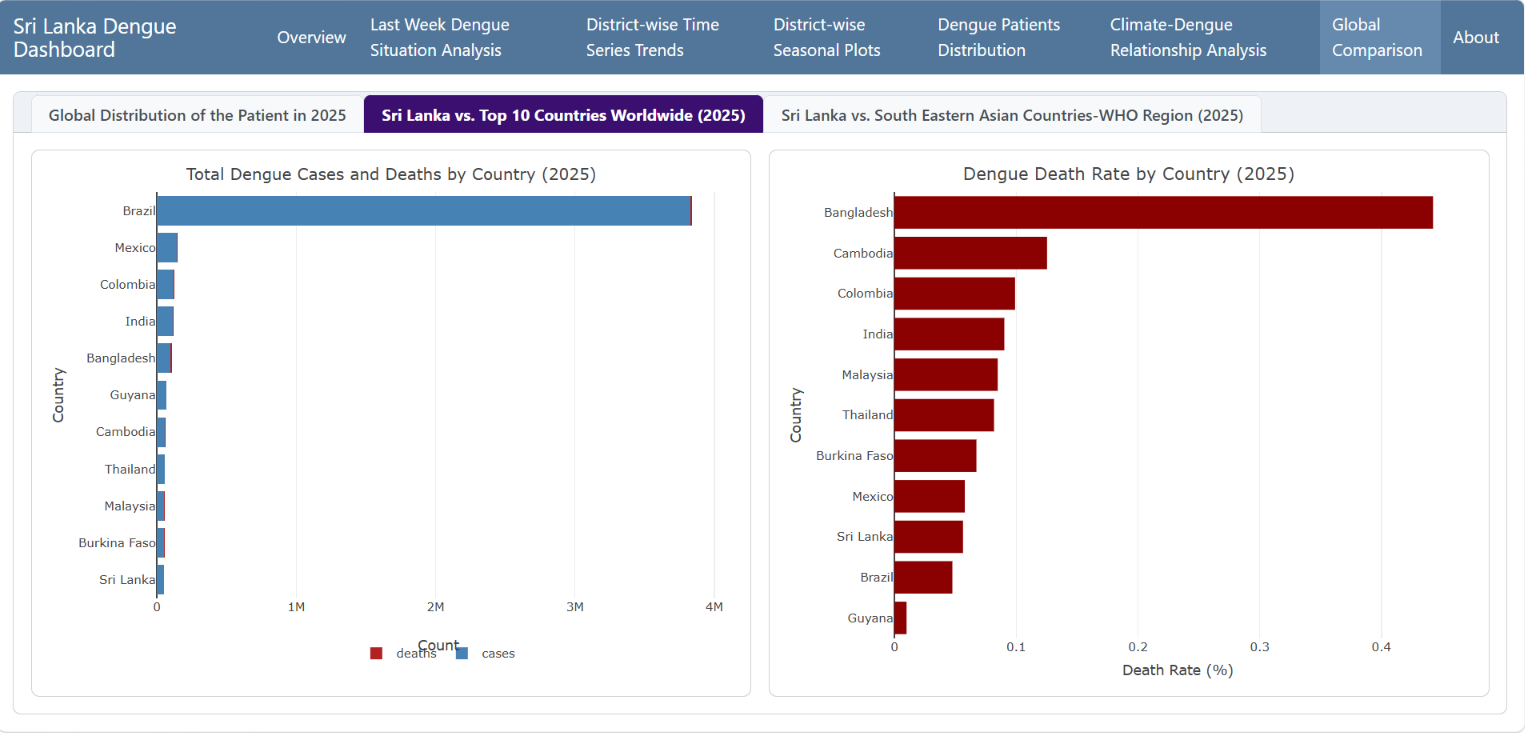
\includegraphics[width=0.98\linewidth,height=\textheight,keepaspectratio]{images/tab7.b.png}

}

\subcaption{\label{fig-tab7-2}}

\end{minipage}%
\newline
\begin{minipage}[t]{0.50\linewidth}

\centering{

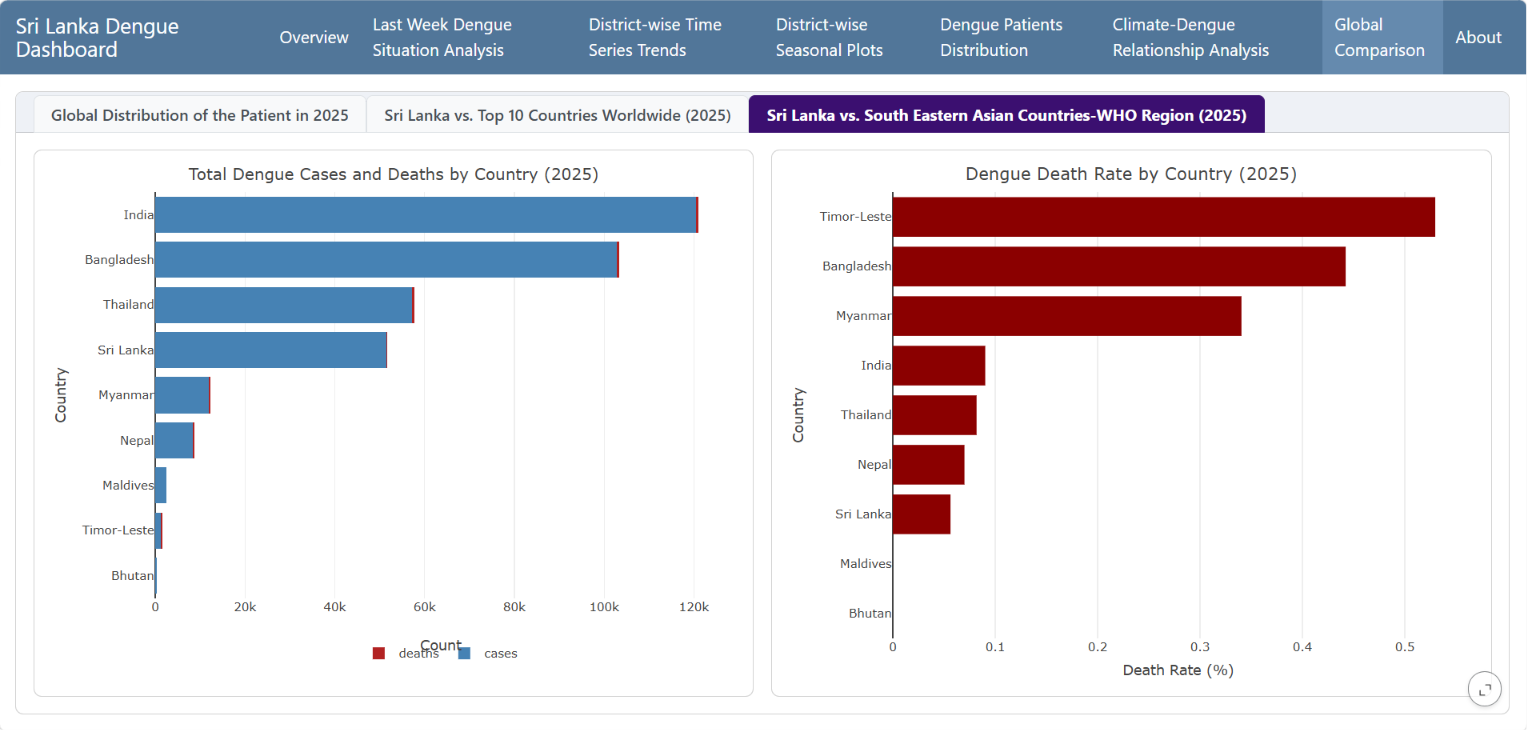
\includegraphics[width=0.98\linewidth,height=\textheight,keepaspectratio]{images/tab7.c.png}

}

\subcaption{\label{fig-tab7-3}}

\end{minipage}%

\caption{\label{fig-tab7}Screenshot of Tab 7 (Global Comparison)}

\end{figure}%

\subsection{Tab 8}\label{tab-8}

\begin{figure}[H]

\centering{

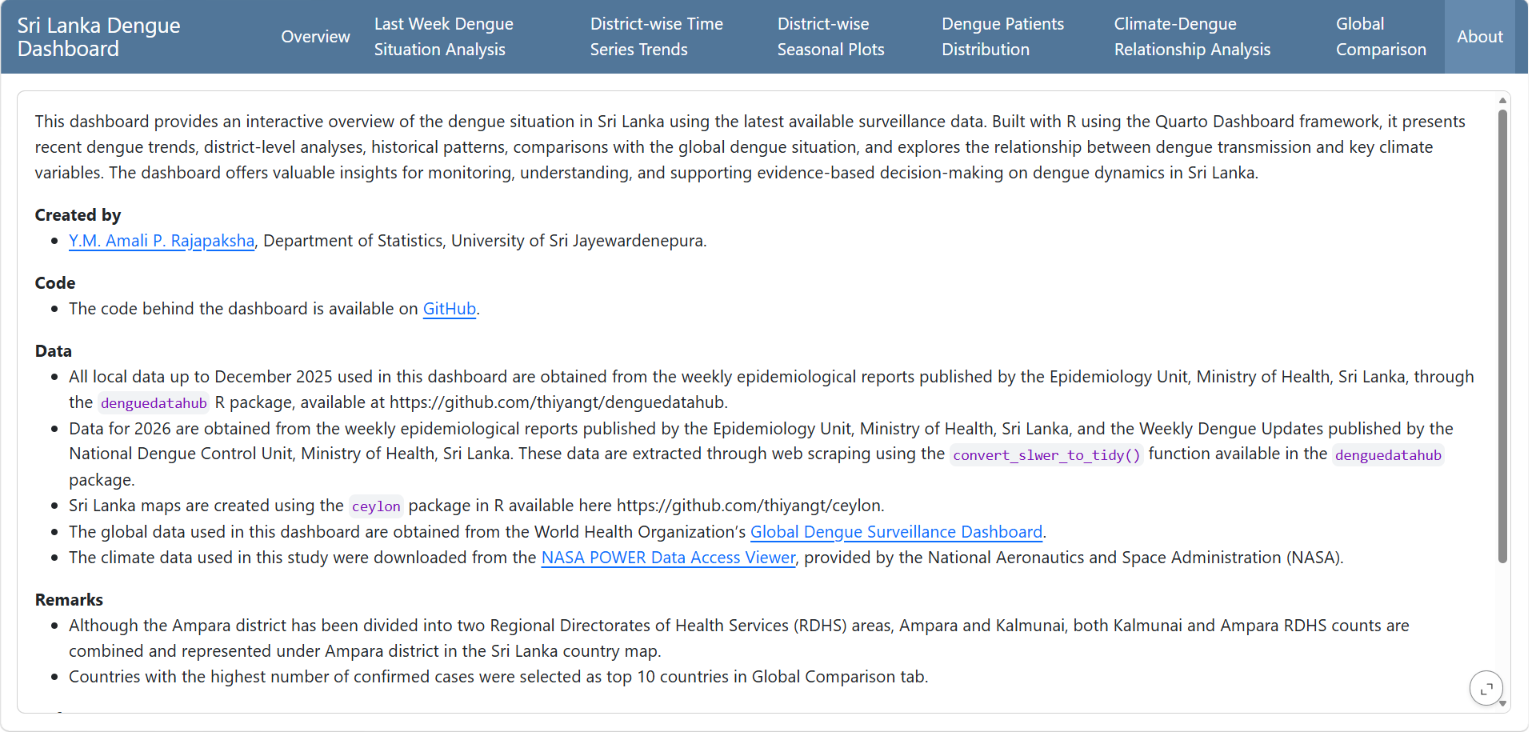
\includegraphics[width=5.1in,height=\textheight,keepaspectratio]{images/tab8.png}

}

\caption{\label{fig-tab8}Screenshot of Tab 8 (About)}

\end{figure}%

The Western Province, particularly the Colombo, Gampaha, and Kalutara
districts, has consistently reported the highest dengue burden in the
country due to high population density, rapid urbanization, construction
activities, environmental conditions favorable for mosquito breeding,
and increased human mobility. Dengue transmission in Sri Lanka
demonstrates a clear seasonal pattern, with two annual peaks
corresponding to the southwest and northeast monsoon periods

From the early 2000s onward, dengue became firmly established as an
endemic disease in Sri Lanka, with cases reported from all districts of
the country. Large epidemics were recorded in 2002, 2004, 2009, 2017,
and 2019. The largest outbreak in Sri Lankan history occurred in 2017,
with more than 186,000 reported dengue cases nationally.




\end{document}
